\documentclass[12pt]{article}
\usepackage{ctex}
\usepackage{amsmath, amssymb}
\usepackage{graphicx}
\usepackage{geometry}
\usepackage{fancyhdr}
\usepackage{float}
\usepackage{color}
\usepackage{booktabs}
\usepackage{caption}
\usepackage{hyperref}
\usepackage{listings}

\geometry{a4paper, margin=1in}

\title{作业十~常微分方程数值解}
\author{PB22000150 刘行}
\date{\today}

\begin{document}

\maketitle

	\section{Adams-Bashforth 5 阶方法求解隐式初值问题}
		\subsection{实验原理}
			本实验考虑如下的初值问题:
			\begin{equation}
				x^{\prime} = \frac{t - e^{-t}}{x + e^{x}}, \quad x\left(0\right) = 0
			\end{equation}
			该方程的解析解由以下隐式关系给出:
			\begin{equation}
				x^{2} - t^{2} + 2e^{x} - 2e^{-t} = 0
			\end{equation}

			目标是在 $t = 1$ 处数值求解 $x\left(1\right)$, 并与由上述隐式方程得到的准确值进行对比, 以评估数值方法的误差.

			我们使用 Adams-Bashforth 五阶显式多步法 (AB5) 进行求解, 该方法基于前五个步长的函数值估计当前点的导数值, 具有五阶精度, 格式如下:
			\begin{equation}
				x_{n+1} = x_{n} + h\left(\frac{1901}{720}f_{n} - \frac{1387}{360}f_{n-1} + \frac{109}{30}f_{n-2} - \frac{637}{360}f_{n-3} + \frac{251}{720}f_{n-4}\right)
			\end{equation}
			其中 $f_{n} = f\left(t_{n}, x_{n}\right)$.

		\subsection{程序思路}
			在实现过程中, 采用四阶 Runge-Kutta 方法 (RK4) 计算前四个点, 以初始化 AB5 方法. 为实现较高精度控制, 我们在每次迭代中使用隐式函数的零点求解来获得精确解, 作为误差参考.

			实验中发现若选取初始点 $x\left(0\right)=0$, 则数值方法得到的解为 $x\left(t\right) = -t$, 并非预计的值. 如图 \ref{fig:f} 左图所示.
			
			因此最终我选取了初值 $x\left(0\right)=1$. 此初值下该方程的解析解由以下隐式关系给出:
			\begin{equation}
				x^2 - t^2 + 2e^x - 2e^{-t} = -1 + 2e
			\end{equation}
			此时的解析解图像如图 \ref{fig:f} 右图所示.

			\begin{figure}[htbp]
				\centering
				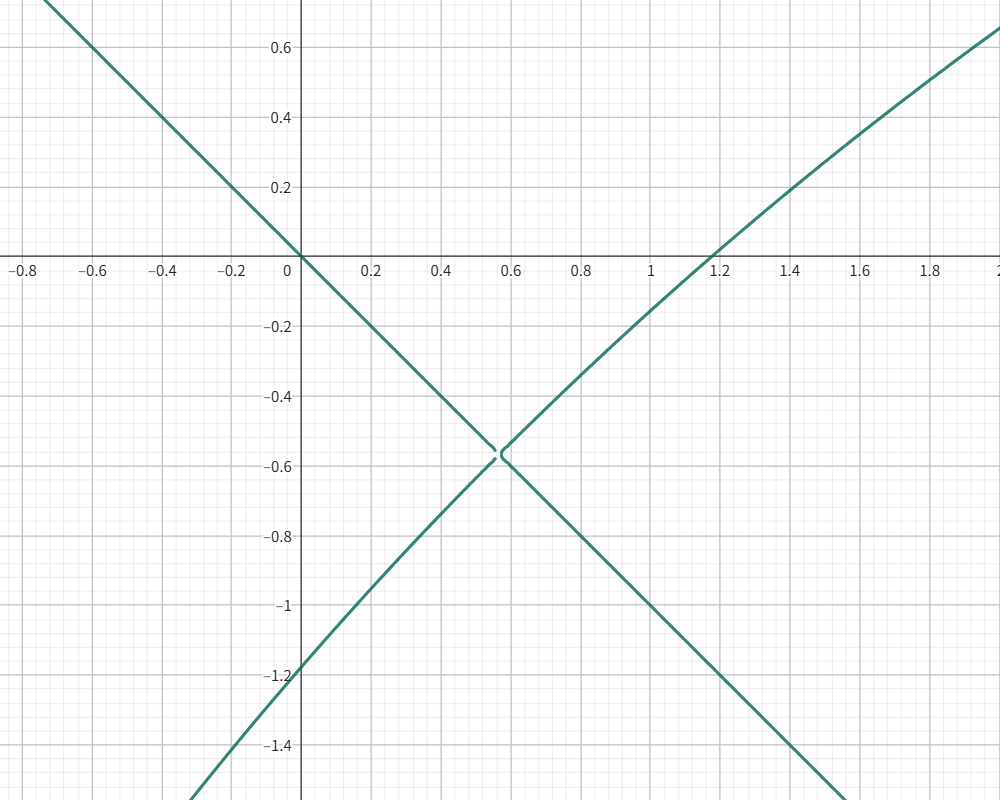
\includegraphics[width=0.45\textwidth]{figure/f_ab50.png}
				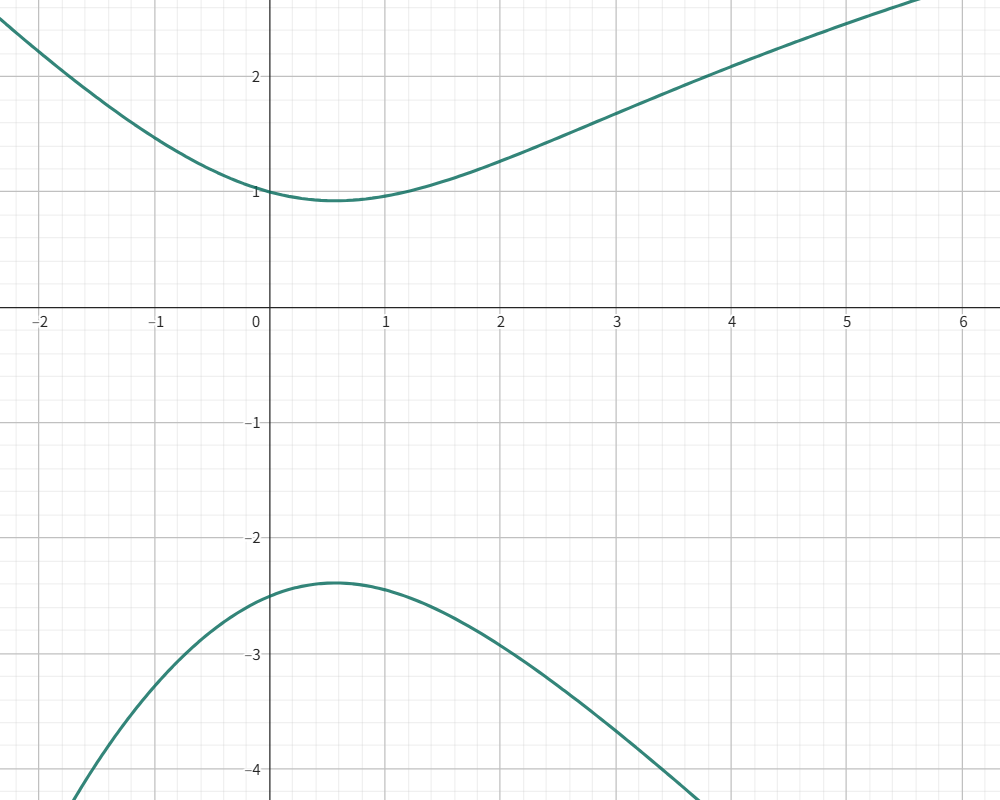
\includegraphics[width=0.45\textwidth]{figure/f_ab51.png}
				\caption{初值 0 与 1 的解析解对比}
				\label{fig:f}
			\end{figure}

		\subsection{实验结果}
			我们选择不同节点数 $N = 2^k,\ k=3,4,5,6,7,8$, 即步长 $h = 1/N$ 进行实验, 得到如下误差与收敛阶:

			\begin{center}
				\begin{minipage}{0.45\textwidth}
					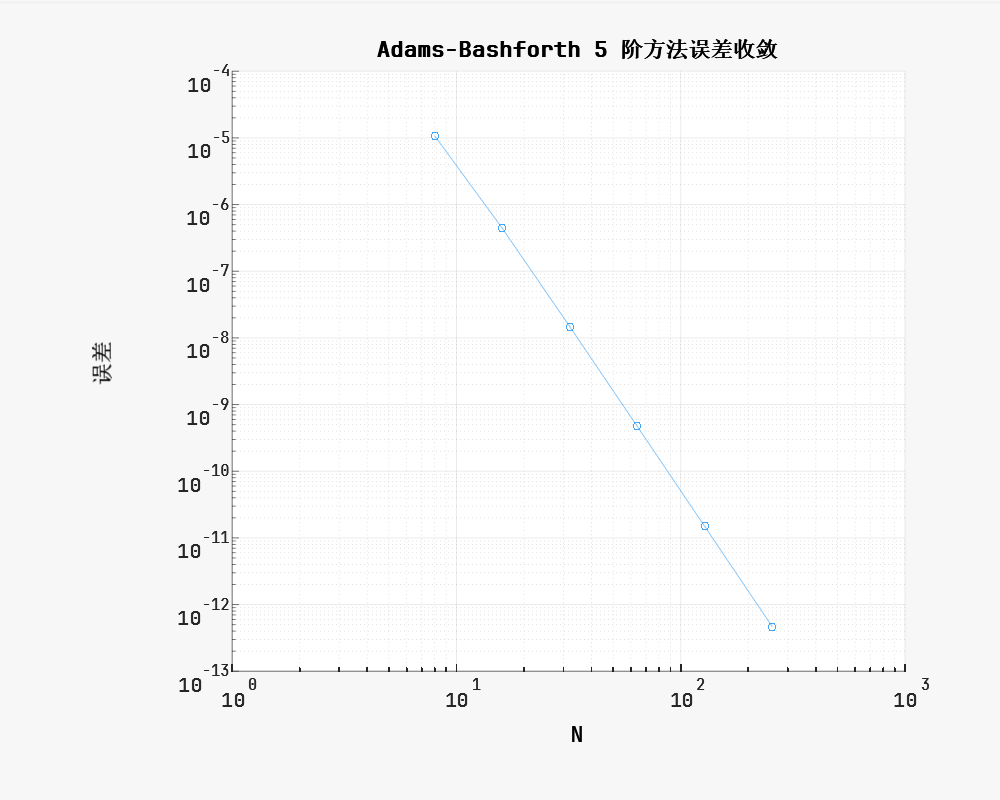
\includegraphics[width=\textwidth]{figure/ab5.png}
				\end{minipage}
				  \hspace{0.05\textwidth}
				\begin{minipage}{0.45\textwidth}
				\begin{verbatim}
	  N           error    order
	  8    1.074802e-05
	 16    4.421001e-07     4.60
	 32    1.477864e-08     4.90
	 64    4.714351e-10     4.97
	128    1.484091e-11     4.99
	256    4.647394e-13     5.00
				\end{verbatim}
				\end{minipage}
			\end{center}

			实验结果表明 AB5 方法在该问题上具有良好的五阶收敛性, 与理论一致.

		\subsection{结果分析}
			从表格和图像中可看出, 随着步长减小, 误差呈现五次方下降趋势. 虽然初始点附近存在一定的数值不稳定性风险, 但在合适精度下不会影响整体收敛. 此外, 使用解析隐式关系构造精确解的方法在验证数值方法时提供了可靠参考.

	\newpage

	\section{自适应 RKF 方法求解微分方程}

		\subsection{实验原理}
			考虑如下常微分方程初值问题:
			\begin{equation}
				y^{\prime} = e^{yx} - \cos\left(y - x\right), \quad y\left(1\right) = 3
			\end{equation}
			该方程具有非线性指数和三角混合结构, 解析解形式未知. 本实验采用 RKF 方法, 即 Runge-Kutta-Fehlberg 方法进行自适应步长积分.

			具体采用 RKF45 或 RKF54 格式, 其中两种不同阶的嵌套公式用于估计局部截断误差, 动态调整步长以控制误差. 我们选择初始步长 $h = 0.01$, 并使用\textbf{第二种步长调整策略}:
			\begin{equation}
				h_{\text{new}} = h \cdot \min\left(\max\left(\text{fac} \cdot {\min}, \text{fac} \cdot \left(\frac{\text{TOL}}{\text{error}}\right)^{1/(p+1)}\right), \text{fac} \cdot {\max}\right)
			\end{equation}
			其中 $\text{fac},\ \text{fac}\cdot{\min},\ \text{fac}\cdot{\max}$ 分别为安全因子和步长限制因子.

		\subsection{程序思路}
			RKF 方法实现时, 必须合理设计误差控制机制, 否则可能导致步长震荡或误判.
			
			在此问题中, 函数 $e^{yx}$ 可能快速增长, 造成数值解爆炸. 对于停止策略,我首先设计了当 \texttt{x+h == x} 时停止, 这是因为最终的求解基于相邻两点的插值, 如果步长已经小于浮点误差, 后面的计算就没有意义了, 计算出的结果不会被调用. 此外我们在计算过程中增加对 \texttt{Inf} 的检测, 若解溢出则自动终止求解.
			
			计算完成会显示解的图像, 可以在 \texttt{rkf\_test.m} 中调用 \texttt{rkf\_adaptive\_solver.m} 时将最后一个参数设为 \texttt{false} 来选择关闭图像显示.

			此外, 用户可以查询任意 $x$ 点的函数值, 通过线性插值实现.

		\subsection{实验结果与图示}
			最终的实验结果如下 (输入了 1.023 作为示例查询点):

			\begin{lstlisting}[mathescape=true]
检测到x无法累加, 终止计算.
解计算完成.
解的范围为 x $\in$ [1.0000, 1.04431288866195570719241914048325]
请输入一个 x $\in$ [1, 1.0443] 查询对应 y 值 (输入回车退出):
1.023
插值结果: y(1.0230) $\approx$ 3.6972146624
			\end{lstlisting}

			绘制的函数图像如下:

			\begin{figure}[htbp]
			\centering
			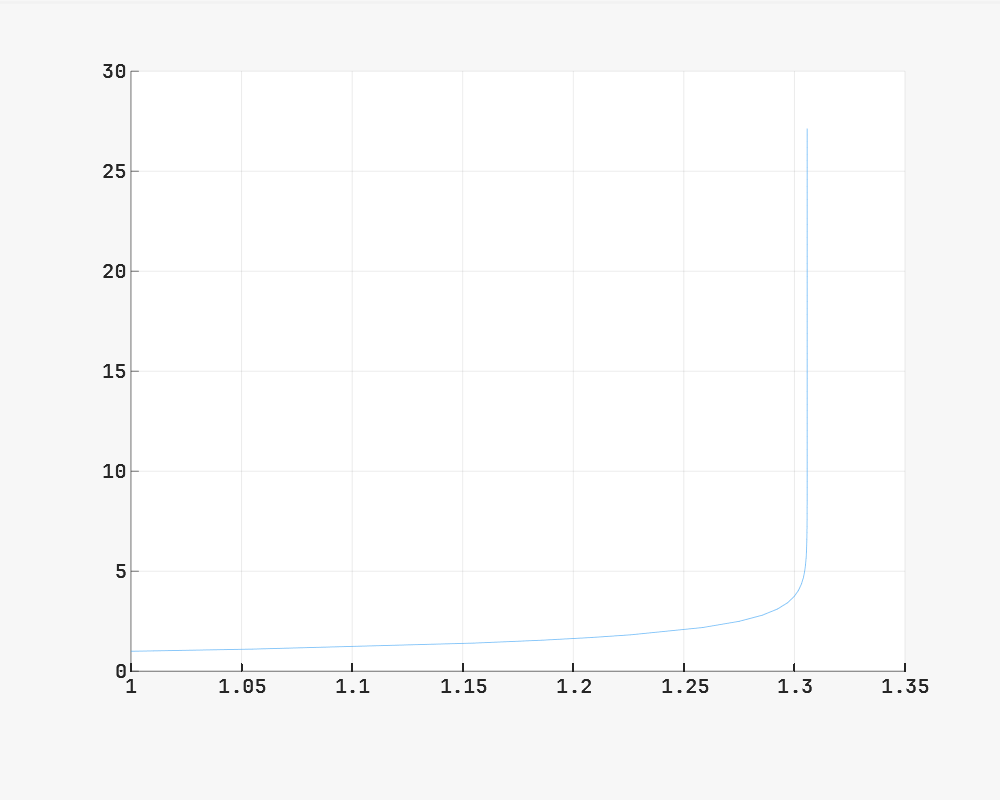
\includegraphics[width=0.7\textwidth]{figure/rkf.png}
			\caption{RKF 方法数值解图像}
			\end{figure}

		\subsection{结果分析}
			该问题数值刚性较强, 指数项增长快, 对误差控制要求高. RKF 方法在短区间内表现稳定, 自动终止机制有效避免了解的无限扩展.  插值机制允许在计算后高效查询任意点函数值, 结合误差估计能保证较高的数值精度. 该方法适用于无解析解的复杂非线性常微分方程求解.

\end{document}
